\begin{figure*}[t]
\centering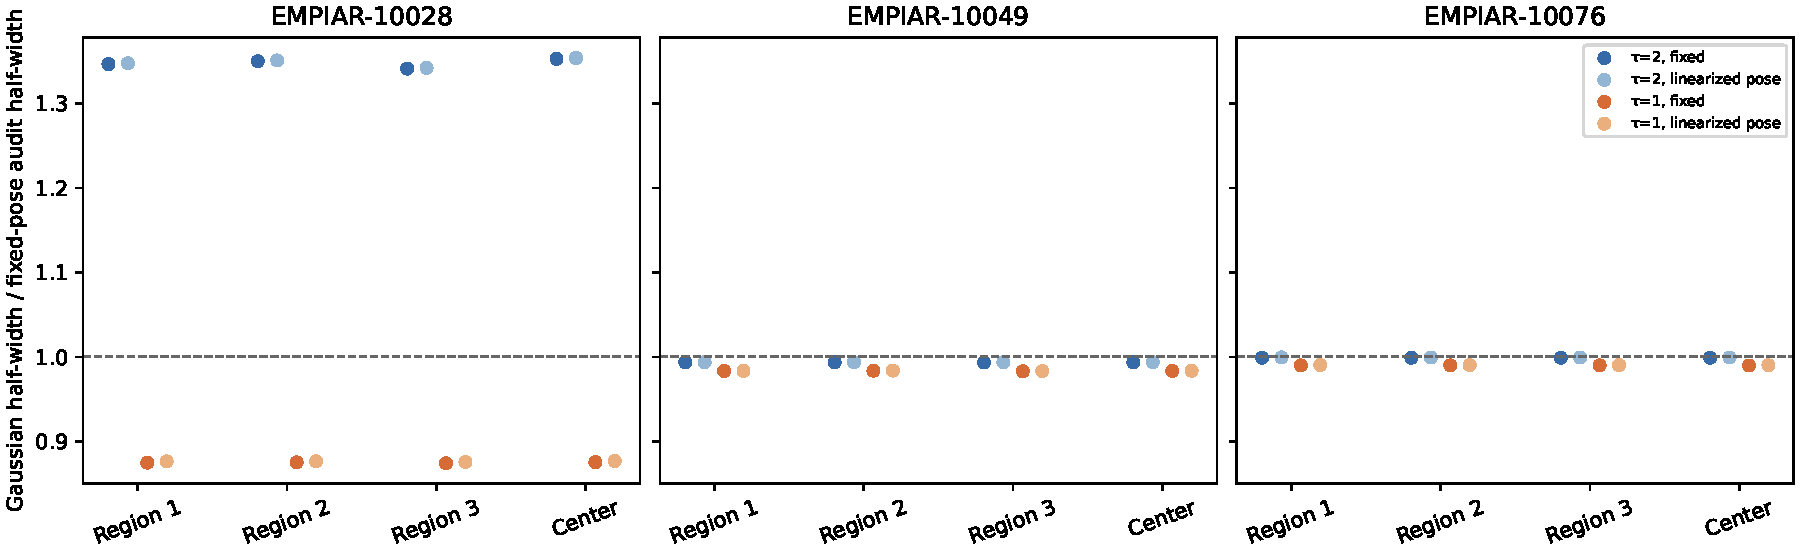
\includegraphics[width=\textwidth]{figures/continuous-gaussian-v2.pdf}
\caption{All twelve locked features and four continuous Gaussian comparisons.
The dashed line denotes the original fixed-pose audit width. Matched prior
scale $\tau=2$ gives near-equal widths on two stacks; its 10028 widths are
34--35\% larger. The half-scale prior is narrower without the same uniform
class implication. Adding the specified first-order Gaussian pose covariance
has little effect here. Every fit converged.}
\label{fig:matchedgaussian}
\end{figure*}
The three complete setup-and-fit runs take 518, 384 and 373 seconds,
respectively, on the authorized Mac under concurrent load. The process peak
resident memory is 6.08 GB; this is a cumulative process high-water mark,
not a fresh per-geometry memory measurement. All relative CG residuals are
at most $9.61\times10^{-11}$. The original rank-1,024 failures are separate
from these 48 successful numerical fits.
